% Field Trip sample script - Documentation - Top level
% Written by Christopher Thomas.

\documentclass[letterpaper,11pt]{report}
\usepackage[letterpaper]{geometry}
\usepackage{graphicx}
\usepackage{verbatim}
\usepackage{placeins}
\usepackage{longtable}

\geometry{nohead,footskip=0.3in,margin=0.75in}

% Force my paragraph style, darnit.
\usepackage{indentfirst}
\setlength{\parskip}{\baselineskip}

% NOTE - "\thispagestyle" is used for part and chapter beginning pages, and
% overrides \pagestyle. Redefine it to be harmless.
% NOTE - The canonical solution ("\pagenumbering{gobble}") resets the page
% counter whenever it's used.
\renewcommand{\thispagestyle}[1]{}

% Custom macros.
\newcommand{\fixme}[1]{\textbf{FIXME: #1}}

\newcommand{\figdef}[3]
{\begin{figure}[htb]
\begin{center}#1\end{center}
\caption{#2}\label{#3}\end{figure}}

\newcommand{\tabdef}[3]
{\begin{table}[hb]
\begin{center}#1\end{center}
\caption{#2}\label{#3}\end{table}}

% Document body.
\begin{document}
%
% Title page.
%
\pagestyle{empty}

\begin{center}
%
\vspace*{1in}
{\Huge Field Trip Test Script -- Code Reference} \\
{\footnotesize Written by Christopher Thomas -- \today.}
%
\vspace*{1in}\\
%
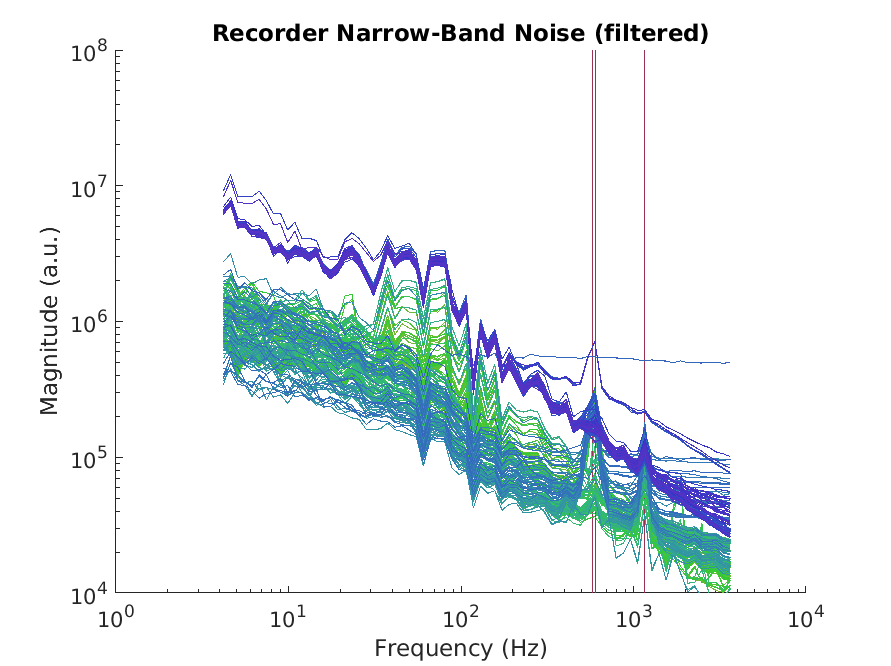
\includegraphics[width=6in]{plots/silicon-noise-spikes-rec}
%
\end{center}
%
\vfill
% FIXME - No license, as this isn't for public release yet.
%{\tiny \input{../../LICENSE.md}}
%
\clearpage
%
%
% Front matter.
%
\pagestyle{plain}
\pagenumbering{roman}
\setcounter{page}{1}
%
\tableofcontents
\clearpage
%
%
% Document parts.
%
\pagestyle{plain}
\setcounter{page}{1}
\pagenumbering{arabic}
%
% Field Trip sample script - Documentation - Overview
% Written by Christopher Thomas.

\chapter{Overview}
\label{sect-over}

This script is designed to test all of the steps involved in reading and
pre-processing experiment data, integrating and aligning data from the
Intan recorder, Intan stimulator, and from USE.

The component scripts are as follows, in the order in which they're called:

\begin{itemize}
%
\item \verb|do_test| is the entrypoint. Edit one line in this file to
select which dataset is processed (the datasets themselves are defined
in a different file).
%
\item \verb|do_test_config| sets configuration parameters. This is the file
that you edit if you want to change how the script processes data.
%
\item \verb|do_test_datasets| defines the datasets that might be processed.
Add new datasets to represent data folders in your own environment.
%
\item \verb|do_test_get_metadata| reads the Field Trip headers for the
ephys data and stores relevant metadata. This also fills in most of the
fields of the configuration structures that will get passed to
\verb|ft_preprocessing|.
%
\item \verb|do_test_autoclassify_chans|, if enabled, reads a short segment
of the recorder and stimulator ephys data and performs signal analysis on
the resulting waveform data. This looks for several things: quantization
noise, narrow-band spectral noise, signal drop-outs, and voltage excursions.
This also performs a power law fit to the LFP spectrum to try to guess
whether a channel contains neural data or noise. Finally, this computes
correlation coefficients between channels to identify groups of channels with
identical data (usually indicating floating channels). The intention of most
of this is to identify "bad" channels in an automated way. The narrow-band
noise information is used to identify beat frequencies that need to be added
to the dataset's notch filter.
%
\item \verb|do_test_align| reads the Unity and SynchBox event data, reads
the ephys TTL data, and builds lists of event codes and reward pulses. Time
alignment tables are generated and used to align event data as well as frame
and gaze data tables from Unity.
%
\item \verb|do_test_process_monolithic|, if enabled, tries to read the
entire ephys dataset and perform signal processing on it. This may optionally
be restricted to a subset of channels and to a shorter time window inside
the dataset. This was mainly used during testing; keep it disabled unless
you actually need it for something, since it takes up a lot of time and RAM.
%
\item \verb|do_test_define_trials| examines the event code sequence and
defines trial boundaries and trigger points based on it. Trials are grouped
into batches, so that trials can be read within a reasonable memory footprint.
%
\item \verb|do_test_process_trials| calls \verb|ft_preprocessing| to read
each batch of trials, performs signal processing on them, extracts aligned
event, frame, and gaze data, and saves all of the associated data series
for each batch of trials to disk.
%
\end{itemize}

Further processing can be performed by reading the trial data and trial
metadata from disk, without having to touch the original data folders.

%
% This is the end of the file.

\input{euscript-fttest-readme}
%
\input{euscript-fttest-topmeta}
\input{euscript-fttest-align}
\input{euscript-fttest-trials}
\input{euscript-fttest-helper}
\input{euscript-fttest-plot}
\input{euscript-fttest-check}
\input{euscript-fttest-mono}
%
%
\end{document}

%
% This is the end of the file.
